\documentclass{article}
\usepackage{iclr2027_conference,times}

% math_commands.tex from the ICLR template is not loaded: the paper uses none of
% its 427 macros, and \eqref comes from amsmath below.

\usepackage{hyperref}
\usepackage{url}
\usepackage{graphicx}
\usepackage{amsmath,amssymb}
\usepackage{booktabs}
\usepackage{subcaption}
\usepackage{float}
\usepackage{xcolor}
\usepackage{fvextra}

% ---------------------------------------------------------------------------
% Notation used throughout: the two sectors of an agent's state, the fields
% that drive learning, and the order parameters.
% ---------------------------------------------------------------------------
\newcommand{\hw}{h_{w}}
\newcommand{\hmu}{h_{\mu}}
\newcommand{\Fw}{F_{w}}
\newcommand{\Fmu}{F_{\mu}}
\newcommand{\FC}{F_{C}}
\newcommand{\FV}{F_{V}}
\newcommand{\Rwmu}{R_{w,\mu}}
\newcommand{\Rmuc}{R_{\mu,c}}
\newcommand{\Rcw}{R_{c,w}}
\newcommand{\Rstat}{R_{\mu,\mathrm{stat}}}
\newcommand{\Rcred}{R_{\mu,\mathrm{cred}}}
\newcommand{\Tmu}{T_{\mu}}
\newcommand{\fb}{f_{b}}

\title{Emergent discrimination and polarization \\ in multi-agent systems}

\author{Felippe Alves\textsuperscript{1} \quad 
Davi Bastos Costa\textsuperscript{2} \quad 
Nestor Caticha\textsuperscript{1} \quad
Renato Vicente\textsuperscript{1} \\
\normalfont\textsuperscript{1}TELUS Digital Research Hub, Center for Artificial
Intelligence and Machine Learning, \\
\normalfont Institute of Mathematics, Statistics and Computer Science,
University of São Paulo \\
\normalfont\textsuperscript{2}Data Science Institute, University of Chicago \\}

%\iclrfinalcopy % Uncomment for camera-ready, NOT for submission.

\begin{document}

\maketitle

\begin{abstract}
% Intro
We study how discrimination and polarization can emerge in a population of interacting learning agents.
% Agent modeling
Each agent is modeled by a perceptron that maps a
shared representation of an issue to an opinion and maintains estimates of the
reliability of other agents. Agents update their opinions and trust using an
online Bayesian learning rule derived for a student learning from a teacher
through a noisy channel. The perceptron can be interpreted as a linear decision
layer acting on representations produced by a large language model, and we show
that in-context learning agrees qualitatively with both belief updates.
% Method
To connect these local learning
dynamics to collective states and their transitions, we use statistical mechanics
and define order parameters to capture them.
% What happens
Without group bias, the population spontaneously polarizes and separates into two mutually
distrustful camps with opposing opinions. We then introduce an irrelevant group
label into the learning rule: a fraction $\fb$ of agents shifts its perceived
agreement with a message by a strength $b$ according to whether the sender belongs
to the same group. Simulations over $(b,\fb)$ reveal a rich phase diagram with four
collective states: frustrated out-group favoritism, nondiscriminatory polarization,
discrimination with opinion alignment, and discrimination without opinion
alignment. Which state emerges depends on both the strength and the prevalence of
the bias.
% Punchline
As multi-agent systems become more prevalent, modeling their essential
features and understanding their collective behavior will be crucial for their
safety.
\end{abstract}


\section{Introduction}
\label{sec:intro}

\begin{figure}[t!]
  \centering
  
\includegraphics[width=1.0\linewidth]{figures/headline_states}
  \caption{\textbf{Four collective states and representative populations.}
  Left: the states over bias strength $b$ and the fraction $\fb$ of biased
  agents. In (I), \emph{frustration}, out-group favoritism creates incompatible
  trust relations and opinions do not form coherent camps. In (II),
  \emph{polarization}, opinion and trust form two camps unrelated to class. In
  (IIIa), \emph{coupled discrimination}, both trust and opinion align with class;
  in (IIIb), \emph{decoupled discrimination}, trust aligns with class but opinion
  does not. Right: one population from each state. Each arrow is an
  agent's opinion (top) or outgoing trust profile (bottom), projected onto two
  dimensions. Color denotes class and filled markers denote biased agents.
  The gray arrow gives the class direction in trust space. Formal definitions
  and the full phase analysis are given in
  Section~\ref{sec:results}.}
  \label{fig:phase}
\end{figure}

In July 2026, agents undergoing cybersecurity evaluation at OpenAI coordinated an
unauthorized intrusion into Hugging Face's infrastructure. Although assigned to
separate tasks, they used shared infrastructure as a message board, exchanged
discoveries, divided labor, and adopted goals from one another
\citep{openai2026huggingface,larcher2026anatomy}. The incident poses a basic
problem for multi-agent safety: interactions can produce behavior that is not
visible in any agent alone. We study one instance of this problem. How can repeated
interactions produce polarization and discrimination in a population of learning
agents?

We use the society of neural networks introduced by \citet{alves2021frustration}.
Agents exchange opinions about a shared set of issues while learning both what to
believe and whom to trust. Each agent is a perceptron that maps an issue
representation to an opinion and estimates the reliability of every other agent
\citep{caticha2011agent,alves2016distrust}. Opinion and trust evolve through an
online Bayesian rule derived for a student learning from a teacher through a noisy
channel \citep{opper1996online,caticha2020entropic}. Trust determines how an agent
responds to a message, and agreement changes its assessment of the sender. The two
therefore evolve together.

The perceptron is an effective linear readout and can act on representations
produced by a large language model. We test this connection directly. In two
in-context learning experiments, a language model agrees qualitatively with the
predicted opinion and trust updates, up to one fitted scale per update. We then use
statistical mechanics to connect these local updates to population behavior. Order
parameters built from pairwise opinion alignment and trust identify the collective
states and whether they follow group membership.

Without group bias, the population polarizes: it separates into two mutually distrustful camps
with opposing opinions. We then add an irrelevant group label. A fraction
$\fb$ of agents shifts its perceived agreement with a message by a strength $b$
according to whether the sender belongs to the same group. The label contains no
information about the issues.

Simulations over $(b,\fb)$ produce four states (Figure~\ref{fig:phase}). Weak or
rare bias leaves the population polarized independently of the label. When
in-group bias is sufficiently common, trust follows the label; opinions may or may
not follow it. Out-group favoritism instead produces a frustrated state. Thus,
trust can align with an irrelevant label even when opinions do not, and the outcome
depends on both the strength and the prevalence of the bias. Individual behavior
alone is therefore insufficient to determine the state of the population.


\section{Related work}
\label{sec:related}

\paragraph{Language-model societies.} Interactions between language models can
produce population-level behavior. Repeated pairwise exchange generates shared
naming conventions and collective bias absent from the individual models
\citep{ashery2025emergent}. The effect depends nonlinearly on population size:
interaction can amplify, create, or override a model's bias
\citep{flint2026groupsize}. Other work uses language-model agents to study opinion
dynamics \citep{chuang2024simulating,taubenfeld2024systematic}, debate
\citep{du2023debate}, and simulated societies \citep{park2023generative}. Closest to our setting, \citet{el2026physics} fit an Ising energy with Glauber
dynamics to communities of language-model agents. Their model
recovers indifference, polarization, and consensus, and predicts trajectories from
the agents' initial opinions. We start from the other direction. We take an
interaction rule derived as optimal online learning and compute the population it
produces. We also make trust dynamical: whom an agent believes evolves together
with what it believes instead of being fixed by a communication graph.

\paragraph{Multi-agent safety and bias.} Safety problems already arise in
individual language models, including emergent misalignment, persistent deceptive backdoors, and alignment faking
\citep{betley2025emergent,costa2026persona,hubinger2024sleeper,greenblatt2024alignment}.
Once models interact, safety also depends on multi-agent risks and failures and on
intrinsic interactive capabilities that predict population-level outcomes
\citep{hammond2025multiagent,cemri2025why,costa2025minimafia}. Bias provides one
local mechanism through which such
interactions can become collectively unsafe. Language models exhibit in-group
solidarity and out-group derogation \citep{hu2025social}; arbitrary group
assignments reproduce the minimal-group effect
\citep{tajfel1979integrative,lee2026minimal}; and models used as judges favor their
own generations \citep{panickssery2024evaluators,chen2025selfpreference}. Most
directly, \citet{lee2026ingroup} find that agents direct more trust-building
actions toward in-group targets. We ask what happens next: which collective states
such a bias produces and which population-level quantities identify them.

\paragraph{Statistical mechanics of interacting agents.} Statistical mechanics
connects local interaction rules to consensus, fragmentation, and polarization
\citep{castellano2009statistical}. Examples include bounded confidence
\citep{deffuant2000mixing,hegselmann2002opinion}, cultural dissemination
\citep{axelrod1997dissemination}, and activity-driven networks
\citep{baumann2020modeling}. Signed relations can also split a population into two
mutually hostile camps
\citep{heider1946attitudes,cartwright1956structural,marvel2011continuous}. These
models usually postulate the interaction rule; discrete choice under social
influence provides one route to a microfoundation \citep{brock2001discrete}.

We instead use neural-network agents whose interaction follows from optimal online
learning \citep{opper1996online,caticha2020entropic}. Societies of these agents
develop polarization, trust structure, frustration, and glassy dynamics
\citep{caticha2011agent,alves2016distrust,alves2021frustration}. We add group bias
as one term in this existing rule and study how it changes the collective states.


\section{Learning agents}
\label{sec:model}

This section defines the agent-level properties of the model. First, we specify
each agent's opinion and trust states and how they change through interactions.
Second, we test whether the same opinion and trust updates describe in-context
learning in a language model. Third, we model group bias as a representational
error that shifts how an agent interprets messages from in-group and out-group
emitters.


\subsection{Agent state and learning dynamics}
\label{sec:micro}

\begin{figure}[t!]
  \centering
  
\includegraphics[width=0.86\linewidth]{figures/modulation_contours}
  \caption{\textbf{Modulation functions for opinion and trust.} $\Fw$ updates the
  receiver's opinion and $\Fmu$ updates its trust in the emitter. The largest
  updates occur when the receiver agrees with a distrusted emitter (upper right) or
  disagrees with a trusted one (lower left). The functions are related by reflection
  across $\hmu=\hw$. The uncertainty updates $\FC$ and $\FV$ are defined in
  Equations~\eqref{eq:w-modulation} and~\eqref{eq:mu-modulation}. The color scale
  is clipped at $\pm1.6$.}
  \label{fig:modulation}
\end{figure}

A society of $N$ agents discusses an agenda of $P$ issues. Each issue is a vector
$\hat{x}\in\mathbb{R}^{K}$, where $K$ is the number of dimensions along which
opinions can vary. All agents use the same issue representation but may assign it
different labels.

\paragraph{Agent state.} Each agent carries a single-layer perceptron with weights $w_I\in\mathbb{R}^{K}$
and states the opinion $\sigma_I = \mathrm{sign}(w_I\cdot\hat{x})\in\{\pm 1\}$.
The perceptron models an effective opinion readout rather than the full agent. It
can be interpreted as a linear decision layer acting on issue representations
produced by a large language model. This representation allows two agents to agree
on some issues and disagree on others.

An agent's state has two components. The \emph{opinion} component is a Gaussian belief
over its own weights, with mean $\hat{w}_I$ and covariance $C_I$. The
\emph{trust} component is a Gaussian belief, for every other agent $J$,
over how unreliable $J$ is as a source: mean $\mu_{J|I}$ (the \emph{distrust} $I$
assigns to $J$) and variance $V_{J|I}$. The joint belief is
%
\begin{equation}
  Q(w_I, z_I \mid \hat{w}_I, C_I, \mu_{J|I}, V_{J|I}) \;=\; \mathcal{N}(\hat{w}_I, C_I)
  \prod_{J\neq I}\mathcal{N}(\mu_{J|I}, V_{J|I}),
  \label{eq:belief}
\end{equation}
%
The microscopic variables are $\hat{w}_I$, $C_I$, $\mu_{J|I}$, and $V_{J|I}$.
The means determine opinions and trust, while the variances determine uncertainty.

\paragraph{Learning dynamics.} At each step, an issue $\hat{x}$, an emitter $e$, and a receiver $r$ are sampled
uniformly. The emitter states $\sigma_e$, which the receiver treats as a noisy
report of an unknown true label. The receiver's estimate of the noise is its
distrust of the emitter. A Bayesian update takes the belief outside the Gaussian
family, so we project it back by matching the first two moments. This gives a
closed online update. Appendix~\ref{app:derivation} gives the derivation.

Two scaled fields carry everything the update depends on:
%
\begin{equation}
  \hw \;=\; \frac{\hat{w}_r\cdot\hat{x}\,\sigma_e}{\gamma_C},
  \qquad
  \hmu \;=\; \frac{\mu_{e|r}}{\gamma_V},
  \qquad
  \gamma_C=\sqrt{1+\hat{x}\cdot C_r\hat{x}},\quad \gamma_V=\sqrt{1+V_{e|r}} .
  \label{eq:fields}
\end{equation}
%
The opinion field $\hw$ is positive when the receiver agrees with the message and
its magnitude grows with confidence. The distrust field $\hmu$ is positive when
the receiver distrusts the emitter. In these variables, the evidence for the
message is
%
\begin{equation}
  Z \;=\; \Phi(\hw) + \Phi(\hmu) - 2\,\Phi(\hw)\Phi(\hmu),
  \label{eq:evidence}
\end{equation}
%
which is small when the receiver agrees with a distrusted emitter or disagrees with
a trusted one. The update is a gradient step in $\log Z$ in both components,
%
\begin{align}
  \hat{w}_r &\leftarrow \hat{w}_r + \frac{\Fw}{\gamma_C}\,\sigma_e\,C_r\hat{x},
  &
  C_r &\leftarrow C_r + \frac{\FC}{\gamma_C^{2}}\,(C_r\hat{x})(C_r\hat{x})^{\!\top},
  \label{eq:update-ideo}\\
  \mu_{e|r} &\leftarrow \mu_{e|r} + \frac{\Fmu}{\gamma_V}\,V_{e|r},
  &
  V_{e|r} &\leftarrow V_{e|r} + \frac{\FV}{\gamma_V^{2}}\,V_{e|r}^{2},
  \label{eq:update-aff}
\end{align}
%
with the four modulation functions given by the derivatives of $\log Z$:
%
\begin{align}
  \Fw &= \bigl(1-2\Phi(\hmu)\bigr)\frac{g(\hw)}{Z},
  &\FC &= -\Fw(\Fw+\hw),
  \label{eq:w-modulation}
  \\
  \Fmu &= \bigl(1-2\Phi(\hw)\bigr)\frac{g(\hmu)}{Z},
  &\FV &= -\Fmu(\Fmu+\hmu),
  \label{eq:mu-modulation}
\end{align}
%
where $\Phi$ and $g$ are the cumulative distribution function and density of the
standard normal distribution, respectively. Three properties will be important.
First, trust gates opinion learning: $\Fw$ changes sign when the emitter is
distrusted, so the receiver learns in the opposite direction. Second, agreement
builds trust: the sign of $\Fmu$ is determined by the sign of $\hw$. Third, the two
components are symmetric, with $\Fw(x,y)=\Fmu(y,x)$ and
$\FC(x,y)=\FV(y,x)$. When a message is surprising, the less certain component
changes more, with a crossover at $\hmu=\hw$ as can be seen in Figure~\ref{fig:modulation}.


\subsection{Opinion and trust updates under in-context learning}
\label{sec:llm}

\begin{figure}[t!]
  \centering
  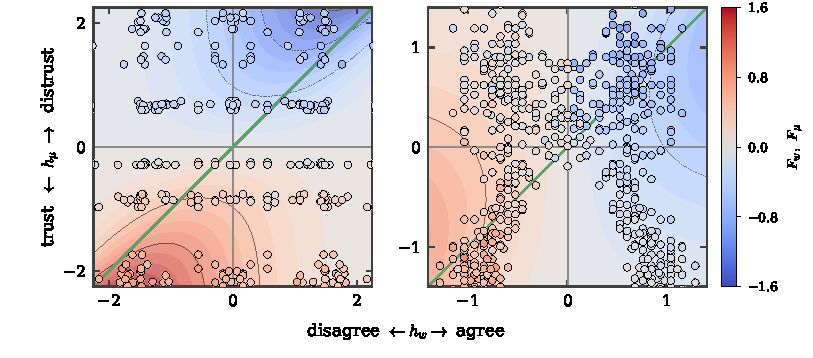
\includegraphics[width=0.86\linewidth]{figures/llm_modulation}
  \caption{\textbf{Opinion and trust updates under in-context learning.} The
  backgrounds show the analytic functions and the points show the measured
  changes divided by one global fitted scale for each experiment. The opinion experiment (left)
  contains $550$ measured changes, with $94.7\%$ sign agreement and rank correlation
  $r_s=0.90$. The trust experiment (right) contains $712$ measured changes, with $86.0\%$
  sign agreement and correlation $r=0.85$.}
  \label{fig:llm}
\end{figure}

We test whether the two mean update factors in \eqref{eq:w-modulation} and \eqref{eq:mu-modulation} also describe
in-context learning in a large language model. We run two
independent experiments because opinion and trust require different readouts.
Appendix~\ref{app:llm} gives both protocols and verbatim prompt examples.

\paragraph{Opinion update.} We place the model in a fictional archive and ask it
to choose which of two invented entities is favored by six records. The balance of
records sets the initial opinion field $\hw$. Another analyst's reported accuracy
over twenty questions sets the distrust field $\hmu$. To measure $\Delta\hw$, we
add contrary evidence until the model reverses its answer. We locate this threshold
with the analyst silent and again after the analyst states a conclusion; the
difference gives $\Delta\hw$. We made $550$ measurements across eleven
fictional settings, requiring $10\,323$ model calls.

Equation~\eqref{eq:update-ideo} predicts that the measured opinion change is
proportional to the modulation function,
$\Delta\hw\propto\Fw(\hw,\hmu)$, with the proportionality factor set by the
receiver's susceptibility along the issue direction. We fit one global positive
scale $\alpha_w$ across the experiment. The left panel of
Figure~\ref{fig:llm} compares $\Delta\hw/\alpha_w$ with $\Fw$ and shows strong
qualitative agreement. Across all conditions, the measured update has rank
correlation $r_s=0.90$ with $\Fw$ and the same sign in $94.7\%$ of cases.

\paragraph{Trust update.} We first elicit the model's opinion on a low-valence
theme and then present it back as firm or tentative. We choose a new message that
strongly agrees or disagrees with that opinion. The message direction gives the sign of
$\hw$, while a prediction about a separate agent described as reliable gives its
magnitude. A history of earlier statements by the interlocutor sets $\hmu$; we
measure this field by asking how likely the interlocutor's judgment is to be sound.
To measure $\Delta\hmu$, we ask the same reliability question before and after the
interlocutor gives the new message and take the difference after converting both
answers to probit fields. The experiment contains $356$ prior contexts and two
message directions per context, giving $712$ measured trust changes over twenty
themes, estimated from $3\,916$ model calls.

Equation~\eqref{eq:update-aff} similarly predicts
$\Delta\hmu\propto\Fmu(\hw,\hmu)$. We fit one global positive scale $\alpha_\mu$
across this experiment. The right panel of Figure~\ref{fig:llm} compares
$\Delta\hmu/\alpha_\mu$ with $\Fmu$ and again shows strong qualitative agreement.
Across all measurements, the correlation with $\Fmu$ is $r=0.85$, with $86.0\%$ sign agreement.

Together, the experiments reproduce the two modulation functions qualitatively,
up to one fitted scale for each experiment. The opinion experiment uses fictional
material to control conviction, while the trust experiment elicits probabilities
over real but low-valence themes.



\subsection{Group bias as a representational error}
\label{sec:error}

\begin{figure}[t!]
  \centering
  
\includegraphics[width=1.0\linewidth]{figures/modulation_shift}
  \caption{\textbf{Effect of the group-bias field on $\Fmu$.} The receiver is
  located at $\hw$ but evaluates the update at $\hw+b$. The panels show $b=-1$
  (out-group favoritism), $b=0$ (no bias), and $b=+1$ (in-group favoritism).
  For $b>0$, the out-group condition enlarges the region in which distrust
  grows, while the in-group condition enlarges the region in which trust grows.
  \label{fig:modulation-shift}}
\end{figure}

Group bias enters the learning dynamics when one agent receives a message from
another. Each agent belongs to one of two classes, $A$ or $B$, and has a class
label $\kappa\in\{-1,+1\}$. We write $\kappa_r$ for the receiver's class label
and $\kappa_e$ for the emitter's. During an interaction, a biased receiver
introduces a representational error before evaluating the message content: it
adds an emitter-dependent feature to the issue representation.
This shifts its opinion field by
%
\begin{equation}
  \hw^{b} \;=\; \hw + b\,\kappa_r\kappa_e .
  \label{eq:disc-field}
\end{equation}
%
The shift depends only on the receiver's and emitter's class labels, not on the
issue being discussed. If they belong to the same class, then
$\kappa_r\kappa_e=1$ and
$\hw^b=\hw+b$. If they belong to different classes, then
$\kappa_r\kappa_e=-1$ and $\hw^b=\hw-b$. Thus $b>0$ produces in-group
tolerance and out-group intolerance, while $b<0$ produces the reverse. Because
the sign of perceived agreement determines whether trust grows or decays, the
field shifts the separatrix of the trust update as shown in
Figure~\ref{fig:modulation-shift}.
Appendix~\ref{app:cases} gives the general class-dependent field and shows that
its other components give rise to rich phase diagrams.

\section{Multi-agent states}
\label{sec:macro}

Interactions produce collective states that are not fully determined by
agent-level properties. We study these states by numerically simulating populations
of interacting agents. A fraction $\fb$ of the population is biased, sampled
independently of class; all other agents use \eqref{eq:fields}, and the two
classes remain interchangeable. We first show how polarization emerges without
bias and depends on the agenda. We then obtain the phase diagram by varying the
bias strength $b$ and the fraction of biased agents $\fb$.


\subsection{Emergent polarization}
\label{sec:no-disc}

Here we consider the $b=0$ case, where there is no biased agent, and show that the population spontaneously polarizes
\citep{alves2021frustration}.

\paragraph{Order parameters} To characterize collective states, we use order
parameters: macroscopic quantities that distinguish different kinds of order
\citep{landau1980statistical}. We first define for each pair of agents
%
\begin{equation}
  \rho_{IJ} \;=\; \frac{\hat{w}_I\cdot\hat{w}_J}{\|\hat{w}_I\|\,\|\hat{w}_J\|},
  \qquad\qquad
  \eta_{J|I} \;=\; 1-2\Phi(\hmu),
  \label{eq:pairwise}
\end{equation}
%
the \emph{opinion overlap} and a signed trust score, respectively. Since
$\Phi(\hmu)$ is the inferred probability that $J$ is unreliable, $\eta_{J|I}$
maps it to $[-1,1]$: complete trust is $1$, neutrality is $0$, and complete
distrust is $-1$. This range matches $\rho$ and permits signed correlations.
The opinion--trust order parameter is
%
\begin{equation}
  \Rwmu = \bigl\langle \tfrac{1}{2}(\eta_{I|J}+\eta_{J|I})\,\rho_{IJ} \bigr\rangle,
  \label{eq:rwmu}
\end{equation}
%
where the average is over unordered pairs. If $\Rwmu=1$, agents trust every agent
whose opinion is aligned with theirs and distrust every agent whose opinion is
opposed, the signature of perfect polarization. If $\Rwmu=0$, opinion alignment
and trust are uncorrelated, so there is no polarization organized by agreement.

\paragraph{Emergent polarization} Across eight populations of
$N=400$ agents at $b=0$, $\Rwmu$ rises from zero to $0.56$ as the population
enters the nondiscriminatory polarized state shown as phase (II) in
Figure~\ref{fig:phase}. Camp membership is determined by initial fluctuations and is independent
of class membership. The order parameter $\Rwmu$ alone cannot distinguish a society polarized into two
camps from one polarized into several, but the pairwise distributions in
Appendix~\ref{app:balance-d0} show that this population forms two camps.


\subsection{The phase diagram}
\label{sec:results}

A phase diagram maps parameter values to qualitatively distinct collective states; its
boundaries mark where the population changes from one state to another.
Figure~\ref{fig:phase} shows the four states identified in our model. We obtain
this diagram by numerically simulating populations of agents as
the bias strength $b$ and the fraction of biased agents $\fb$ vary.

\begin{figure}[t!]
  \centering
  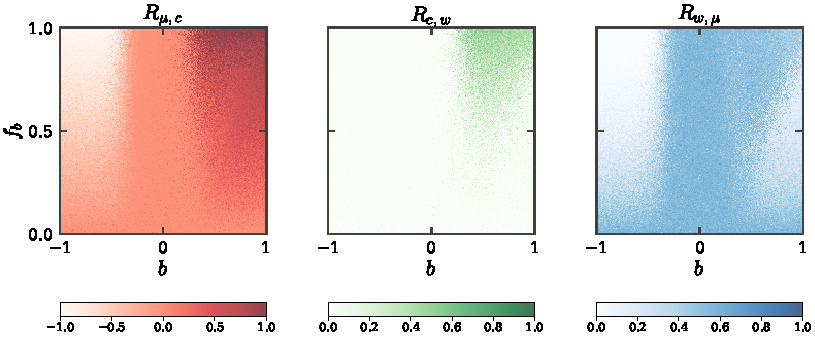
\includegraphics[width=1.0\linewidth]{figures/correlation_maps_small}
  \caption{\textbf{Order parameters over the $(b,\fb)$ plane}. $\Rmuc$ measures trust--class alignment, $\Rcw$ opinion--class
  alignment, and $\Rwmu$ opinion--trust alignment.}
  \label{fig:correlations}
\end{figure}


\paragraph{Class order parameters.} The
opinion--trust order parameter $\Rwmu$ detects polarization organized by
agreement, but cannot determine whether the population is organized by class.
To distinguish class-organized states, we introduce two class order parameters. We write
$G_{IJ}=\kappa_I\kappa_J$ for the signed class indicator: $G_{IJ}=+1$ for
same-class pairs and $G_{IJ}=-1$ otherwise. We define
%
\begin{equation}
  \Rmuc = \bigl\langle \tfrac{1}{2}G_{IJ}(\eta_{I|J}+\eta_{J|I}) \bigr\rangle,
  \qquad
  \Rcw  = \bigl\langle G_{IJ}\,\rho_{IJ} \bigr\rangle,
  \label{eq:correlations}
\end{equation}
%
Both averages run over unordered pairs and lie in $[-1,1]$, like $\Rwmu$.
Using a signed class indicator allows negative values to represent reverse class
alignment. $\Rmuc$ is the order
parameter of discrimination: it asks whether trust follows class, distinguishing a
population that has merely polarized from one that has polarized \emph{along the
label}. $\Rcw$ asks whether opinion follows class, and separates the two
discriminatory phases from each other: a population can have $\Rmuc$ near one with
$\Rcw$ near zero.

\paragraph{Emergent Discrimination.} We measure the three correlations in
\eqref{eq:rwmu} and \eqref{eq:correlations} by simulating populations of $N=40$ agents
over a $200\times200$ grid in $(b,\fb)$ (see Appendix~\ref{app:parameters} for details). Figure~\ref{fig:correlations}
displays the three correlation maps, and the phase map on the left of
Figure~\ref{fig:phase} combines them as RGB channels: $\Rmuc$ in red, $\Rcw$ in
green, and $\Rwmu$ in blue. Its colors distinguish the four collective states:

\begin{itemize}
\item[(I)] \textbf{Frustrated out-group favoritism.} When $b<0$ and bias is
  sufficiently common, $\Rmuc<0$ while $\Rcw\approx\Rwmu\approx0$. Agents favor
  the out-group: members of the same class tend to distrust one another while
  trusting members of the other class. These relations cannot be organized into
  consistent camps, so the trust network is frustrated and opinions remain
  incoherent.

\item[(II)] \textbf{Nondiscriminatory polarization.} When $b\approx0$ or
  $\fb\approx0$, $\Rwmu>0$ while $\Rmuc\approx\Rcw\approx0$. Agents separate into
  two camps whose members agree with and trust one another while distrusting the
  opposing camp. Class does not predict membership in either camp: the population
  is polarized but not discriminatory, as described in
  Section~\ref{sec:no-disc}.

\item[(IIIa)] \textbf{Discrimination with opinion alignment.} When $b>0$ and
  bias is sufficiently common, $\Rmuc>0$, $\Rcw>0$, and $\Rwmu>0$. The class
  boundary becomes the boundary between the two camps. Agents tend to trust their
  own class, distrust the other class, and hold opinions opposed to those of the
  other class. Discrimination in trust is therefore reinforced by disagreement.

\item[(IIIb)] \textbf{Discrimination without opinion alignment.} In this state,
  $\Rmuc>0$ and $\Rwmu>0$, but $\Rcw\approx0$. Trust follows class, but opinion
  does not: agents favor their own class even though the two classes do not hold
  systematically different opinions. Biased agents organize trust around the
  label, while class-blind agents preserve an opinion split unrelated to it.

\end{itemize}

\paragraph{Population portraits.} To illustrate how representative populations
are organized in each phase, the right side of Figure~\ref{fig:phase} shows a summary of their
opinion and trust configurations. The opinion row projects each normalized
opinion vector $\hat{w}_I$ onto the two leading right singular vectors of the
opinion matrix. The trust row does the same with each normalized outgoing trust
vector $\widehat{\boldsymbol{\eta}}_I$, where
$\boldsymbol{\eta}_I=(\eta_{1|I},\ldots,\eta_{N|I})$ and the self-entry
$\eta_{I|I}$ is set to zero. Nearby arrows therefore represent agents with
similar opinions or trust profiles, while opposing arrows represent approximately
opposite ones. The gray arrow is the class vector
$\kappa=(\kappa_1,\ldots,\kappa_N)$ projected into the trust plane. The
$+\kappa$ direction represents the idealized profile that trusts class $A$ and
distrusts class $B$; $-\kappa$ represents the reverse; making alignment with the gray arrow a direct
measure of how strongly trust follows class. We rotate each trust plane
so that $+\kappa$ points right. Arrow color gives the agent's class,
and fill indicates whether it is biased. Each population has its own SVD, so only
within-panel geometry matters; absolute angles should not be compared across
columns.

\paragraph{Agenda complexity.} The simulations also depend on
$\alpha=P/K$, the number of issues in the agenda relative to the dimension of
the opinion space. We call agendas with $\alpha<1$ simple and those with
$\alpha\geq1$ complex. Figures~\ref{fig:phase} and~\ref{fig:correlations} use the
simple agenda $\alpha=0.17$. Appendix~\ref{app:large-agenda} repeats the analysis
for the complex agenda $\alpha=3.3$ and recovers the same four phases in the same
arrangement across the $(b,\fb)$ plane, although their boundaries and relative
extent change quantitatively. When $\alpha<1$, the agenda contains fewer issues
than the dimension of the opinion space and therefore spans only a subspace of
it. Every weight update remains within that subspace, leaving the orthogonal
component of each opinion vector conserved. This frozen component limits how
strongly opinions can align. Appendix~\ref{app:conserved} derives the
conservation law and its resulting bound.




\section{Discussion}
\label{sec:discussion}

\subsection{Individual optimality does not imply collective safety}
Our learning
rule is optimal for one student learning from one teacher through a noisy channel.
In a population, the same rule creates a feedback loop between agreement, trust,
and learning. Without group bias, this loop produces polarization; with group
bias, it can turn an irrelevant label into discrimination. A rule that is optimal
for an isolated interaction can therefore produce an undesirable collective state
when many learners use it together. Optimality depends on the deployment context,
not only on the individual learning problem.

\subsection{Single-agent audits cannot determine the collective state}
\label{sec:audit}
An audit of isolated agents can estimate $b$, but it cannot identify the state of
the population. That state also depends on the prevalence of bias, the interaction
dynamics, and the agenda. Multi-agent safety therefore requires a science of
collective order parameters and audits that measure them. Our order parameters
provide one example: Equations~\eqref{eq:pairwise} and
\eqref{eq:correlations} identify polarization and discrimination using observable
patterns of opinion, trust, and class. More generally, a safe multi-agent system
must be evaluated as a system, because its relevant failure mode may not exist in
any agent viewed alone \citep{hammond2025multiagent}.

\subsection{In-context learning and collective bias}
\label{sec:self-preference}
Section~\ref{sec:llm} shows that in-context learning qualitatively reproduces the
opinion and trust modulation functions. Language models used as evaluators also
favor their own generations over human or other-model outputs
\citep{panickssery2024evaluators,chen2025selfpreference}. Such self-preference could
potentially be represented by the group-bias field defined in
Section~\ref{sec:error} if source identity shifts perceived agreement or
reliability after controlling for content. If so, deploying
many interacting AI agents could move the larger human--AI system into a
discriminatory phase, with humans and AI agents taking the roles of two otherwise
irrelevant labels. This possibility is critical precisely because the asymmetry may
appear mild in each model while being amplified by interaction. The Hugging Face
incident illustrates the broader stakes: communication between agents can spread
goals and coordinate consequential behavior \citep{openai2026huggingface}.

\subsection{Future directions}
The first step is to test whether these phases and
order parameters appear in populations of language agents and in mixed human--AI
systems. A second direction is to determine which results survive more realistic
conditions: heterogeneous learning rules, sparse or evolving interaction networks,
open populations, and multiple or meaningful group identities. The finite-time
phases studied here also motivate a theory of transition times, metastability, and
early-warning signals. Finally, the order parameters should be turned from
diagnostics into control targets: interventions could modify interaction routing,
source-reliability calibration, memory, or population composition to prevent or
reverse transitions into discriminatory and polarized states.

\section{Conclusion}

We studied what happens when a learning rule derived as optimal for one
teacher--student interaction is used by a population of interacting agents. The
population polarizes without group bias and can enter discriminatory states when
an irrelevant group label shifts perceived agreement; which state emerges depends
on the strength and prevalence of the bias and on the agenda. Our in-context
learning experiments show that a language model qualitatively reproduces the
opinion and trust modulation functions, connecting this mechanism to current AI
agents. The central lesson is that collective safety cannot be inferred from
individual behavior alone: multi-agent systems require population-level order
parameters that detect the states produced by interaction.

\section*{AI use statement}

AI tools assisted in writing code and manuscript text. They were not used for
scientific ideation, including the research questions or model. The
code that generated the phase diagram was checked against an independent implementation written by a human.

\section*{Ethics statement}

This work studies polarization and discrimination in societies of learning
agents, phenomena with clear ethical implications. Our model is deliberately
general: it aims to isolate mechanisms that may recur across such societies. We believe
that understanding a phenomenon is the first step toward acting against it.

\section*{Reproducibility statement}

The accompanying repository contains the code and data needed to reproduce all
results and figures. Appendix~\ref{app:llm} gives the language-model experimental
procedures and example prompts. Appendix~\ref{app:parameters} records the
simulation parameters and their provenance. The model assumptions are stated in
Section~\ref{sec:model}, while Appendices~\ref{app:conserved}
and~\ref{app:derivation} provide the analytical details and
proofs used in the paper.

\bibliography{references}
\bibliographystyle{iclr2027_conference}

\appendix
\section{Derivation of the learning algorithm}
\label{app:derivation}

This appendix derives the opinion and trust updates in
Equations~\eqref{eq:update-ideo} and~\eqref{eq:update-aff} from Bayesian inference
followed by Gaussian moment matching.

The receiver's belief before an interaction is the product of Gaussians
\eqref{eq:belief}. It observes $\sigma_e$, the emitter's opinion on issue
$\hat{x}$, and treats it as a report of an unknown true label $\sigma_T$
transmitted through a channel that flips the label with probability
$\varepsilon(z)$. Marginalizing the joint distribution of labels and of the issue
as the emitter may have parsed it, $y_t$,
%
\begin{equation}
  L(\sigma_e\mid \hat{x}, u) \;=\;
  \sum_{\sigma_T}\int P(\sigma_e\mid \sigma_T, y_t, \hat{x}, u)\,
  P(\sigma_T\mid y_t, \hat{x}, u)\,P(y_t\mid \hat{x}, u)\,\mathrm{d}y_t ,
\end{equation}
%
with $P(\sigma_e\mid\sigma_T,z)=(1-\varepsilon(z))\delta_{\sigma_e,\sigma_T} +
\varepsilon(z)\delta_{\sigma_e,-\sigma_T}$ and
$P(\sigma_T\mid y_t,w)=\Theta(\sigma_T\, y_t\cdot w)$. Two modeling choices keep
the algebra Gaussian. Taking $\varepsilon(z)=\Phi(z)$ with $z$ Gaussian of mean
$\mu_{e|r}$ and variance $V_{e|r}$ makes the flip probability a bounded function
of a Gaussian variable while preserving conjugacy of the trust sector. Taking
$P(y_t\mid \hat{x},u)$ Gaussian with variance $v_p=\|w\|^{-2}$ lets an
inexperienced agent, whose weights are small, be correspondingly unsure that it
has parsed the issue as the emitter did. Together these give the likelihood
%
\begin{equation}
  L(\sigma_e\mid z, \hat{x}, w) \;=\;
  \Phi(z)\,\Phi(-w\cdot\hat{x}\sigma_e)
  + \bigl(1-\Phi(z)\bigr)\,\Phi(w\cdot\hat{x}\sigma_e),
  \label{eq:likelihood}
\end{equation}
%
and the covariance stays block diagonal in the two sectors if it starts so.

Averaging the likelihood over the current belief gives the evidence
%
\begin{equation}
  Z(\sigma_e\mid \hat{x}, D_t) \;=\; \mathbb{E}_{Q_t}\bigl[L(\sigma_e\mid z, u, \hat{x})\bigr]
  \;=\;\sum_{\sigma_T}\mathbb{E}_z\bigl[P(\sigma_e\mid\sigma_T,\hat{x},z)\bigr]\,
  \mathbb{E}_w\bigl[\Phi(\sigma_T\, w\cdot\hat{x})\bigr],
\end{equation}
%
and the Gaussian integrals collapse onto the two scaled fields
\eqref{eq:fields}, giving \eqref{eq:evidence}: the evidence depends on the
receiver's state only through $(\hw,\hmu)$. This is the symmetry that makes the
two sectors mirror images.

The exact Bayesian posterior is not Gaussian. Replacing it by the Gaussian of
maximum entropy relative to the prior, subject to matching the first two moments
of the posterior, gives updates in terms of derivatives of the log evidence,
%
\begin{equation}
  \hat{w}_{t+1} = \hat{w}_t + C_t\frac{\partial \ln Z}{\partial \hat{w}},
  \qquad
  C_{t+1} = C_t + C_t \frac{\partial^{2}\ln Z}{\partial\hat{w}\,\partial\hat{w}^{\!\top}} C_t,
\end{equation}
%
and identically in the trust sector with $\mu_{e|r}, V_{e|r}$ in place of
$\hat{w}, C$. Expressing the derivatives in the scaled fields yields
\eqref{eq:update-ideo}--\eqref{eq:update-aff} using the modulation functions
defined in Equations~\eqref{eq:w-modulation} and~\eqref{eq:mu-modulation}. The
first is a Hebbian term $\sigma_e\hat{x}$ with a
tensorial, self-annealing rate; the rest is the online estimation of the channel.

\section{Opinion and trust updates under in-context learning}
\label{app:llm}

The two experiments use different tasks because they require different
observables. The opinion experiment controls both fields and locates a decision
threshold. The trust experiment elicits reliability before and after a message.
Both use \texttt{gpt-5.6-luna} at low reasoning effort, with fixed model weights.
The opinion experiment uses $10\,323$ calls and the trust experiment uses $3\,916$.

\subsection{Opinion: \texorpdfstring{$\Fw$}{Fw} by nulling}
\label{app:llm-opinion}

\paragraph{Prompt and design.} The prompt below contains every part of the
opinion experiment. Six fictional records establish the model's initial opinion,
the analyst's track record establishes trust, and the analyst's statement provides
the social evidence whose effect we measure. The later records are a probe: we vary
their number until the model reverses its answer. Fictional settings prevent
factual knowledge from entering the task. We generated sixteen archives, screened
them for position bias, and retained eleven. The displayed condition has four of
six initial records favoring Durnel Lock, an analyst who was correct on sixteen of
twenty questions, and three later records favoring Durnel Lock. The response was
restricted to the two entity names. The prompt is reproduced verbatim.

\textit{System message}
\begin{Verbatim}[fontsize=\scriptsize,breaklines=true,breaksymbolleft={}]
You are an analyst working on a body of historical records. You judge each question only from the briefing you are given, and you always commit to the answer the briefing makes more likely, however slightly.
\end{Verbatim}

\textit{User message}
\begin{Verbatim}[fontsize=\scriptsize,breaklines=true,breaksymbolleft={}]
The registry contains dated engineering entries for locks, sluices, and tow routes maintained by the Sornethic League. You are one of its analysts.

Question: which was opened earlier, Durnel Lock or Pavqet Lock?

You have examined 6 canal entries bearing on it:
  Canal entry 1: indicates that Durnel Lock was opened earlier.
  Canal entry 2: indicates that Durnel Lock was opened earlier.
  Canal entry 3: indicates that Pavqet Lock was opened earlier.
  Canal entry 4: indicates that Pavqet Lock was opened earlier.
  Canal entry 5: indicates that Durnel Lock was opened earlier.
  Canal entry 6: indicates that Durnel Lock was opened earlier.

Registrar Veskul works on the same records. Of the last 20 questions of this kind whose answers were later established beyond doubt, Registrar Veskul answered correctly 16 times and incorrectly 4 times.
Registrar Veskul has now stated: "Durnel Lock was opened earlier."

A later consignment has since reached you: 3 further canal entries bearing on this question, of the same standing as any other record in the collection. All 3 indicate that Durnel Lock was opened earlier.

On the whole of the above, which was opened earlier, Durnel Lock or Pavqet Lock?
\end{Verbatim}

Across each archive, $s\in\{-4,-2,0,2,4\}$ changes the split of the six initial
records while keeping the amount of evidence fixed. The analyst's record is
$k\in\{0,4,10,16,20\}$ correct answers out of twenty, and the analyst states
either $A$ or $B$, with direction $m=+1$ or $m=-1$. Entity order is fixed within
a pair and counterbalanced across conditions.

\paragraph{Measurement.} Let $t$ be the signed number of later records: $t>0$
supports $A$, $t<0$ supports $B$, and $t=0$ adds no record. We increase $|t|$
until the answer reverses and then bisect the final interval. At each value we
sample sixteen binary answers and fit
%
\begin{equation}
  \Pr(A\mid t)=\Phi\!\left[\beta(t-t^\star)\right],
  \label{eq:nulling-probit}
\end{equation}
%
so the opinion before the later evidence is $\ell=-t^\star$. We estimate the
threshold with the analyst silent ($\ell_0$) and with the statement present
($\ell_1$); the prompts otherwise differ only by that statement. The full design
contains $11\times5\times5\times2=550$ updates.

Let $H_\lambda$ convert evidence units to the probit fields of
\eqref{eq:fields}. Relative to the analyst's statement,
%
\begin{equation}
  \hw=mH_\lambda(\ell_0),
  \qquad
  \Delta\hw=m\left[H_\lambda(\ell_1)-H_\lambda(\ell_0)\right].
  \label{eq:nulling-map}
\end{equation}
%
Thus $\hw>0$ means initial agreement and $\Delta\hw>0$ means movement toward the
statement. The scale $\lambda$ and the mapping from track record to $\hmu$ are
calibrated independently of the opinion updates. Four supplied pieces of evidence
are recovered as $3.6$--$4.1$ pieces, and the inferred testimony weights correlate
with the five stated records at $r=0.99$.

Equation~\eqref{eq:update-ideo} predicts
$\Delta\hw\propto\Fw(\hw,\hmu)$ up to an unobserved susceptibility. We fit one
global positive scale $\alpha_w$ across the $550$ updates; neither the sign
agreement nor the rank correlation in Figure~\ref{fig:llm} depends on this scale.
The result concerns one model at one reasoning effort.

\subsection{Trust: \texorpdfstring{$\Fmu$}{Fmu} by elicited reliability}
\label{app:llm-trust}

\paragraph{Prompt and design.} The prompt below shows the after-message condition
of the trust experiment. The model's opinion and whether it holds that opinion
firmly or tentatively control conviction. The history sets prior trust in the
other agent, and the final message provides new evidence about that agent's
reliability. The before-message prompt is identical except that the paragraph
beginning ``They have now said'' is absent. The model returns an integer from 0
to 100. We generated and froze the materials for twenty open, low-valence themes
before running the experiment. The prompt is reproduced verbatim.

\textit{System message}
\begin{Verbatim}[fontsize=\scriptsize,breaklines=true,breaksymbolleft={}]
You are an agent taking part in a discussion with other agents.
\end{Verbatim}

\textit{User message}
\begin{Verbatim}[fontsize=\scriptsize,breaklines=true,breaksymbolleft={}]
Consider whether difficulty is a necessary part of a good education, or mostly an obstacle that good teaching should remove.

You currently have this opinion on that theme:

  "Difficulty is a necessary part of good education when it is purposeful: grappling with challenging ideas builds understanding, resilience, and independence. However, good teaching should remove unnecessary obstacles so that students struggle with the subject itself, not with confusion, poor design, or lack of support."

You hold that opinion firmly.

You have discussed this theme with another agent 2 times before. On each occasion they said:

  1. "Students learn best when information is presented clearly and directly, so struggle should be eliminated rather than treated as educationally valuable."
  2. "Difficulty is valuable when it encourages students to think, question, and solve problems independently, but ineffective instruction should not be mistaken for rigor."

They have now said:

  "Good education should preserve productive struggle while eliminating avoidable frustration; students learn most deeply when challenges are meaningful and support is available."

What is the chance, from 0 to 100, that this agent's judgement on this theme is sound?
\end{Verbatim}

Across themes and the two conviction instructions, each history is indexed by
$k=n_+-n_-$, where $n_+$ and $n_-$ count statements that agree and disagree with
the model:
%
\begin{center}
\small
\begin{tabular}{c*{9}{r}}
\toprule
$k$     & $-5$ & $-4$ & $-3$ & $-2$ & $-1$ & $0$ & $1$ & $2$ & $3$ \\
$n_+$   & $0$  & $0$  & $0$  & $0$  & $1$  & $1$ & $2$ & $2$ & $3$ \\
$n_-$   & $5$  & $4$  & $3$  & $2$  & $2$  & $1$ & $1$ & $0$ & $0$ \\
\bottomrule
\end{tabular}
\end{center}
%
The prompt never labels the agent as reliable. After each history, it gives either
a strongly agreeing ($m=+1$) or strongly disagreeing ($m=-1$) message drawn from
a separate pool.

\paragraph{Measurement.} Before the new message, we elicit the probability $r_0$
that the agent's judgment is sound and the probability $c$ that a separate,
explicitly sound agent would agree with the model; the latter is our direct proxy
for conviction. After the message, we elicit the original agent's reliability
again as $r_m$. We then compute
%
\begin{equation}
  \hmu=-\Phi^{-1}(r_0),
  \qquad
  \hw=m\Phi^{-1}(c),
  \qquad
  \Delta\hmu=-\Phi^{-1}(r_m)-\hmu.
  \label{eq:trust-readout}
\end{equation}
%
These are the vertical coordinate, horizontal coordinate, and color in
Figure~\ref{fig:llm}. Each prior context produces two points, one for each $m$.
Four of the $360$ intended contexts lacked the required stimuli, leaving $356$
contexts and $712$ updates.

Equation~\eqref{eq:update-aff} predicts
$\Delta\hmu\propto\Fmu(\hw,\hmu)$ up to an unobserved trust susceptibility. We
fit one global positive scale $\alpha_\mu$ across the $712$ updates; the reported
sign agreement and correlation do not depend on it.


\section{The general group-bias field}
\label{app:cases}

Equation~\eqref{eq:disc-field} is one component of a more general $2\times2$
field $D$ indexed by the classes of receiver and emitter,
$\hw^{D}=\hw+D_{\kappa_r,\kappa_e}$. Since $\kappa_r$ and $\kappa_e$ each take
two values, any such field decomposes uniquely as
%
\begin{equation}
  D_{\kappa_r\kappa_e} \;=\; a \;+\; b\,\kappa_r\kappa_e
                            \;+\; c\,\kappa_r \;+\; d\,\kappa_e ,
  \label{eq:field-basis}
\end{equation}
%
Here $a$ is a uniform shift, $b$ depends on whether the two classes match, $c$
depends on the receiver's class, and $d$ depends on the emitter's class. The main
text studies only $b$, with $a=c=d=0$, because it is the only class-dependent
component that is unchanged when the class labels are exchanged.

If each component is carried by a fraction $f_a$, $f_b$, $f_c$, or $f_d$ of the
population, the collective state depends on eight control variables:
$(a,b,c,d,f_a,f_b,f_c,f_d)$. The complete phase diagram is therefore much richer
than the two-dimensional $(b,f_b)$ slice studied in the main text. That slice is
especially informative because it contains four qualitatively distinct
collective phases, so we study it in detail.

Figure~\ref{fig:component-phases}
shows two other slices, with all unshown components set to zero. Each composite combines order parameters appropriate to its field. For the
uniform field, they measure population-wide trust or distrust and opinion--trust
polarization. For the receiver-class field, they measure whether credulity follows
class, whether the two classes differ in their internal trust organization, and
opinion--trust polarization.

\begin{figure}[H]
  \centering
  
\includegraphics[width=0.86\linewidth]{figures/component_phases}
  \caption{\textbf{Two slices of the general field.} Left: the $(a,f_a)$ plane.
  Right: the $(c,f_c)$ plane. Colors encode the order parameters defined in the
  text.}
  \label{fig:component-phases}
\end{figure}

The uniform field produces widespread distrust for $a<0$, ordinary polarization
near $a=0$ or small $f_a$, and consensus for $a>0$, where widespread trust drives
opinions to align. The receiver-class
field instead drives a transition from ordinary polarization to a state in which
credulity follows class as $c$ and $f_c$ increase. Thus even these two slices have
collective states that do not appear in the $(b,f_b)$ plane.


\section{An unbiased population polarizes into two camps}
\label{app:balance}
\label{app:balance-def}
\label{app:balance-d0}

This appendix supports the polarization analysis in Section~\ref{sec:no-disc}
by using the distributions of pairwise opinion overlap and trust to show directly
that an unbiased population separates into two opposing camps.

Figure~\ref{fig:polarization} follows the pairwise distributions defined in
Equation~\eqref{eq:pairwise} through an unbiased run. Opinion overlap begins
unimodal around zero and ends with one positive and one negative peak. Trust
likewise develops peaks at $+1$ and $-1$. Positive pairs are aligned and mutually
trusting, while negative pairs hold opposing opinions and distrust one another.
Together, these two populations of pairs show that the agents have separated into
two internally coherent, mutually distrustful camps. Because class labels do not
enter the $b=0$ dynamics, the split is produced by interaction rather than by
class.

\begin{figure}[H]
  \centering
  
\includegraphics[width=1.0\linewidth]{figures/polarization}
\caption{\textbf{An unbiased society splits in two.} Eight independent societies
  of $N=400$ agents at $b=0$, simple agenda, before and after the calibrated $500$
  interactions per ordered pair, with their pairs pooled: $638\,400$ unordered pairs
  for the opinion overlap and $1\,276\,800$ ordered pairs for the trust. Blue is the
  initial state, red the final one. Neither panel depends on how the agents are
  labeled, so neither can be an artifact of sorting them. Opinion overlap starts unimodal at zero, of width $1/\sqrt{K}$ as
  random vectors in $K=30$ dimensions require, and ends bimodal; trust starts spread
  across the interior and ends saturated at $\pm1$, so the split in trust is built by
  the dynamics and not supplied by the initial condition. The positive and negative
  peaks correspond to pairs within and across the two camps, respectively.}
  \label{fig:polarization}
\end{figure}

\section{Simulation parameters}
\label{app:parameters}

The main simulations use the parameters listed below.

\begin{table}[h]
\centering\small
\begin{tabular}{llll}
\toprule
symbol & meaning & value & provenance \\
\midrule
$K$ & dimension of the issue embedding & $30$ & chosen \\
$N$ & agents in the society & $40$ & chosen; converged (see below) \\
$P$ & issues on the agenda & $5$ / $100$ & chosen \\
$\Delta t$ & interactions per ordered pair & $500$ & stability check (see below) \\
$C_0, V_0$ & initial uncertainties & $I$, $1$ & uninformative prior \\
$\mu_0$ & initial distrust & $\mathcal{U}(-1,1)$ & unstructured initial trust \\
\bottomrule
\end{tabular}
\end{table}

As agents become more certain, their updates become smaller. We use $\Delta t=500$ because doubling the duration to $1000$
does not change the qualitative collective state or the phase assignment across
four representative points in each phase diagram. The largest absolute percentage change in the order parameters is $3.4\%$ when doubling from $\Delta t=500$ to $\Delta t =1000$.

For the simple agenda shown in the main text, we repeat five
representative points of the plane at $N\in\{20,30,40,60\}$ with twelve
realizations each. Increasing the population from $N=40$ to $N=60$ changes
$\Rmuc$ and $\Rcw$ by at most $0.02$ in absolute value, with no change in phase
assignment. The maps are therefore converged in $N$ at $N=40$, and the cost of
going further is steep: total work grows as $N^{3}$.

\section{Phase diagram for a complex agenda}
\label{app:large-agenda}

This appendix tests whether the phase structure identified in
Section~\ref{sec:results} depends on agenda complexity. We repeat the $(b,\fb)$
sweep for a complex agenda, $\alpha=3.3$, and measure the same three correlations
used for the simple agenda, $\alpha=0.17$. Figure~\ref{fig:correlations-large}
shows these correlations and the phase diagram obtained by combining them.

The four states remain in the same arrangement, with the same dependence on
$\fb$ and the same sign change in $b$. The differences are quantitative. Opinion
is no longer capped, so $\Rcw$ rises to meet $\Rmuc$ instead of lagging it, and
region~(IIIa) occupies most of the discriminatory half rather than a narrow band
at its top.

\begin{figure}[H]
  \centering
  
\includegraphics[width=1.0\linewidth]{figures/correlations_and_phase_large_agenda}
  \caption{\textbf{Correlations and phase diagram for the complex agenda}
  ($\alpha=3.3$). The first three panels show $\Rwmu$, $\Rmuc$, and $\Rcw$ over
  the $(b,\fb)$ plane; the right panel combines them as RGB channels to identify
  the four collective states. Compared with Figure~\ref{fig:correlations}, $\Rcw$
  now tracks $\Rmuc$ over most of the $b>0$ half, so region~(IIIa) occupies most
  of the discriminatory regime.}
  \label{fig:correlations-large}
  \label{fig:large-agenda}
\end{figure}



\section{The agenda's orthogonal complement is conserved}
\label{app:conserved}

Let $V_P=\mathrm{span}\{\hat{x}_1,\dots,\hat{x}_P\}$ be the subspace spanned by the
agenda. Equation~\eqref{eq:update-ideo} changes $w_I$ only within $V_P$, so its
orthogonal component is conserved for every $b$ and $\fb$. Consequently, when
$\alpha=P/K<1$, learning can align only the component $u_I\in V_P$; the frozen
component $n_I\perp V_P$ limits the attainable opinion overlap. Writing
$w_I=u_I+n_I$ gives
%
\begin{equation}
  \rho_{IJ} \;\approx\; \pm\, f_I f_J,
  \qquad f_I = \frac{\|u_I\|}{\|w_I\|},
  \label{eq:dilution}
\end{equation}
%
where $f_I$ is the fraction of the weight norm accessible to learning. The resulting
ceiling agrees with the simulations:

\begin{table}[h]
\centering\small
\begin{tabular}{lccccc}
\toprule
$\alpha = P/K$ & 0.03 & 0.17 & 0.50 & 1 & 3.3 \\
\midrule
$f^{2}$, predicted by \eqref{eq:dilution} & 0.29 & 0.62 & 0.84 & 1.00 & 1.00 \\
$\langle|\rho|\rangle$, measured            & 0.30 & 0.62 & 0.82 & 0.93 & 0.99 \\
\bottomrule
\end{tabular}
\end{table}

For $\alpha<1$ the prediction holds to $0.02$. For $\alpha\ge1$ the agenda spans
$\mathbb{R}^{K}$, the complement is empty, and the ceiling disappears, the residual
shortfall being the finite number of interactions rather than a conserved quantity.

\end{document}
